\documentclass[12pt]{article}
\usepackage{amsmath}
\usepackage{graphicx}
\usepackage{float}
\usepackage[utf8]{inputenc}
\usepackage{cite}
\usepackage{setspace}
\usepackage{amsfonts}
\usepackage{mathrsfs}
\usepackage[margin=1.0in]{geometry}
\usepackage{enumitem}
\usepackage{listings}

\numberwithin{equation}{section}

\title{Numerical Solutions to the Problem of the Solar System}
\author{Elizabeth Drueke}

\begin{document}
\maketitle

\begin{abstract}
The study of the solar system is a good window into how planetary bodies orbit and interact.  As a result, determining numerical methods for solving for the orbits of planets in the Milky Way have broad applications in many areas of astrophysics.  Here, we work on developing two such methods -- the Verlet and 4th-order Runge-Kutta algorithms -- and apply them to the problem of our solar system, focusing particularly on stability of orbits and computation time required to do the calculations. 
\end{abstract}

\section{Introduction}
\label{sec:intro}

For as long as humans have been on the earth, we have been looking to the sky.  Ancient peoples relied on the stars and planets to tell when the seasons were changing, so they would know when was a good time to plant crops for food.  A little later, the stars were used by mariners as a compass, guiding them across the seas.  
\\\indent Today still we look towards the skies.  However, we arguably know more about them.  We know that our solar system is not the center of the universe, nor are we the center of our solar system.  We know that our sun is a middle-sized star, and without its light and heat there would be no life on earth.  We know that the rotation of the planets around the sun is dictated by Newton's Second Law, and, with this, we can calculate the trajectory of the planetary bodies around us.  
\\\indent Here, we present two such calculations.  Using the Verlet and $4^{th}$-Order Runge-Kutta (RK4) Methods, we investigate the motion of the planets around the sun.  We begin by presenting the simple theory of planetary motion in Section~\ref{sec:theory}.  Then we discuss the Verlet and RK4 methods in Sections~\ref{subsec:verlet} and~\ref{subsec:rk4}.  After this, we discuss the framework and the algorithm developed particularly in this project in Section~\ref{sec:algorithm}.  Finally, results and benchmarks for the code are discussed in Section~\ref{sec:results}.

\section{Theory}
\label{sec:theory}

As mentioned in Section~\ref{sec:intro}, the movements of planets are dictated by Newton's Second Law, which states

$$\vec{F} = m\vec{a}.$$

\noindent Thus, we have a second order differential equation:

$$m\frac{d^{2}\vec{x}}{dt^{2}} = \vec{F}$$

\noindent where $\vec{F}$ is the sum of the forces on the planet in question.  In particular, the force of one planet on another is given by

\begin{equation}
\label{eq:bigg}
\vec{F} = -\frac{Gm_{1}m_{2}}{r^{2}}\hat{r}
\end{equation}

\noindent where $G = 6.67\times10^{-11} m^{3}kg^{-1}s^{-2}$ is the gravitational constant, $m_{1,2}$ are the masses of the two planets, and $r$ is the distance between the planets.
\\\indent Now, we want to be able to use some sort of discretized version of this in order to use a computer to approximate a numerical solution to this problem.  Our first step is then to look at Eq.~\ref{eq:bigg} component-wise (ie. look at the $x$- and $y$- components separately).  In particular, we should have

$$
m\frac{d^{2}x}{dt^{2}} = F_{x} \text{ and } m\frac{d^{2}y}{dt^{2}} = F_{y}
$$

\noindent Noting that $\vec{r}=x\hat{x}+y\hat{y}$, this gives us that

$$
F_{x} = -\frac{Gm_{1}m_{2}x}{r^{3}}\text{ and } F_{y} = -\frac{Gm_{1}m_{2}y}{r^{3}}
$$

\noindent Thus we have two coupled second-order differential equations:

\begin{equation}
\label{eq:diffeqs1}
\frac{d^{2}x}{dt^{2}} = -\frac{Gm_{1}x}{r^{3}}\text{ and } \frac{d^{2}y}{dt^{2}} = -\frac{Gm_{1}y}{r^{3}}
\end{equation}

\noindent or, alternatively, four coupled first-order differential equations:

\begin{equation}
\label{eq:diffeqs2}
\begin{align}
\frac{dx}{dt} = v_{x} &\text{, }&\frac{dv_{x}}{dt}=-\frac{Gm_{1}x}{r^{3}}, \\
\frac{dy}{dt} = v_{y} &\text{, }&\frac{dv_{y}}{dt}=-\frac{Gm_{1}y}{r^{3}}.
\end{align}
\end{equation}

\\\indent In this analysis, we first investigate the unperturbed earth-sun system.  In this case, Eq.~\ref{eq:bigg} becomes

\begin{equation}
\label{eq:earthsunbigg}
\vec{F} = \frac{GM_{\odot}m_{E}}{r^{2}}\hat{r}
\end{equation}

\noindent where $m_{E}$ is the mass of the earth and $M_{\odot}$ is the mass of the sun.  Assuming a circular orbit, we can say that 

$$a = \frac{mc^{2}}{r},$$

\noindent and so we have

$$\frac{mv^{2}}{r} = \frac{GM_{\odot}m_{E}}{r^{2}}$$

\noindent or

$$v^{2}r = GM_{\odot} = 4\pi^{2} AU^{2}yr^{-2}.$$

\noindent Thus, for the unperturbed earth-sun system, we wish to investigate

\begin{equation}
\label{eq:earthsun}
\frac{d^{2}x}{dt^{2}} = -\frac{4\pi^{2}x}{r^{3}} \text{ and } \frac{d^{2}y}{dt^{2}} = -\frac{4\pi^{2}y}{r^{3}}.
\end{equation}

\\\indent We will also want to look at adding other planets to our solar system.  After all, the unperturbed earth-sun system is really to simplistic too be a reasonable approximation for how the solar system evolves in time.  Noting that

$$Gm_{p} = GM_{\odot}\frac{m_{p}}{M_{\odot}}=4\pi^{2}\frac{m_{p}}{M_{\odot}},$$

\noindent we have, for planet $p\prime$,

\begin{equation}
\label{eq:multiplanet}
\begin{align}
a_{x} &=  \frac{dv_{x}}{dt} =&  -\frac{4\pi^{2}}{r_{p\prime\odot}^{3}}\left(x_{p\prime} - x_{\odot}\right) - \frac{4\pi^{2}}{M_{\odot}}\sum_{p\neq p\prime}\frac{m_{p}\left(x_{pprime} - x_{p}\right)}{r_{pp\prime}^{3}}, \\
a_{y} &=  \frac{dv_{y}}{dt} =&  -\frac{4\pi^{2}}{r_{p\prime\odot}^{3}}\left(y_{p\prime} - y_{\odot}\right) - \frac{4\pi^{2}}{M_{\odot}}\sum_{p\neq p\prime}\frac{m_{p}\left(y_{p\prime} - y_{p}\right)}{r_{pp\prime}^{3}}.
\end{align}
\end{equation}

\\\indent The solution of Eq.~\ref{eq:earthsun} is fairly straightforward (we are only really looking at two coupled second-order differential equations), although still not simple by any means.  However, the solution to Eq.~\ref{eq:multiplanet} is impossible to calculate by hand.  The number of couple equations will be twice the number of planets in the solar system.  Thus, to solve either system, it is useful to turn to numerical approximations and computer algorithms.  In particular, we look into the Verlet and RK4 methods as means by which to solve the system.

\subsection{Verlet Method}
\label{subsec:verlet}

It is a common practice in creating computer algorithms to solve complex problems to discretize the equations in order to get something more concrete to work with.  In this case, we will discretize using the Taylor Series expansion.  That is, 

\begin{equation}
\label{eq:taylor}
x\left(t+h\right) = x\left(t\right)+hx^{'}\left(t+h\right)+\frac{h^{2}}{2}x^{'}^{'}\left(t+h\right)+O\left(h^{3}\right)
\end{equation}

\noindent Thus, we can say, letting $x_{i} = x\left(t_{0}+hi\right)$, that, for planet $p\prime$ in the multi-planet system, 

\begin{equation}
\label{eq:discx}
\begin{align}
x_{i+1} &= x_{i}+hv_{i}+\frac{h^{2}}{2}v_{i}^{'}+O\left(h^{3}\right) \\
&= x_{i}+hv_{i}+\frac{h^{2}}{2}\left(-\frac{4\pi^{2}}{r_{p\prime\odot}_{i}^{3}}\left(x_{p\prime}-x_{\odot}\right)_{i} - \frac{4\pi^{2}}{M_{\odot}}\sum_{p\neq p\prime}\frac{m_{p}\left(x_{p\prime}-x_{p}\right)_{i}}{r_{pp\prime}_{i}^{3}}\right)+O\left(h^{3}\right).
\end{align}
\end{equation}

\noindent We can similarly discretize the velocity of planet $p\prime$ to find

\begin{equation}
\label{eq:discv}
\begin{align}
v_{i+1} &= v_{i}+\frac{h}{2}\left(v_{i+1}^{'}+v_{i}^{'}\right)+O\left(h^{2}\right) \\
&= v_{i}+\frac{h}{2}\left(-4\pi^{2}\left(\frac{\left(x_{p\prime}-x_{\odot}\right)_{i}}{r_{p\prime\odot}_{i}^{3}}+\frac{\left(x_{p\prime}-x_{\odot}\right)_{i+1}}{r_{p\prime\odot}_{i+1}^{3}}\right) \\
 &- \frac{4\pi^{2}}{M_{\odot}}\sum_{p\neq p\prime}m_{p}\left(\frac{\left(x_{p\prime}-x_{p}\right)_{i}}{r_{pp\prime}_{i}^{3}} +  \frac{\left(x_{p\prime}-x_{p}\right)_{i+1}}{r_{pp\prime}_{i+1}^{3}}\right)\right)+O\left(h^{3}\right).
\end{align}
\end{equation}

\noindent In the case of the unperturbed earth-sun system, Eqs.~\ref{eq:discx} and~\ref{eq:discv} simplify to

$$
x_{i+1} =  x_{i}+hv_{i}+\frac{h^{2}}{2}\left(-\frac{4\pi^{2}}{r_{p\prime\odot}_{i}^{3}}\left(x_{p\prime}-x_{\odot}\right)_{i}\right)+O\left(h^{3}\right)
$$

\noindent and

$$
v_{i+1} =  v_{i}+\frac{h}{2}\left(-4\pi^{2}\left(\frac{\left(x_{p\prime}-x_{\odot}\right)_{i}}{r_{p\prime\odot}_{i}^{3}}+\frac{\left(x_{p\prime}-x_{\odot}\right)_{i+1}}{r_{p\prime\odot}_{i+1}^{3}}\right)\right)+O\left(h^{3}\right).
$$

\\\indent Together, Eqs.~\ref{eq:discx} and~\ref{eq:discv} make up what is known as the Verlet method [4].  With the introduction of the velocity Verlet method, this method is self-starting.

\subsection{Fourth-Order Runge-Kutta}
\label{subsec:rk4}

The RK4 method is a bit more precise than the Verlet method discussed in Section~\ref{subsec:verlet}.  It is based on the observation that, for

$$
\frac{dy}{dt} = f\left(t,y\right),
$$

\noindent we can say

$$
y\left(t\right) = \int f\left(t,y\right)dt.
$$

\noindent Discretizing, this yields

$$
y_{i+1}=y_{i} + \int_{t_{i}}^{t_{i+1}}f\left(t,y\right)dt.
$$

\noindent Letting $y_{i+1/2} = y\left(t_{i}+h/2\right)$, and using the midpoint formula for the integral, we find 

$$
\int_{t_{i}}^{t_{i+1}}f\left(t,y\right)dt \approx hf\left(t_{i+1/2},y_{i+1/2}\right)+O\left(h^{3}\right).
$$

\noindent Thus, we have

$$
y_{i+1}=y_{i} +  hf\left(t_{i+1/2},y_{i+1/2}\right)+O\left(h^{3}\right).
$$

\noindent However, it is clear that, in order to use this method, we must have some idea of what $y_{i+1/2}$ is.  To get this quantity, we use Euler's method to approximate it:

$$
y_{i+1/2} \approx y_{i}+\frac{h}{2}f\left(t_{i},y_{i}\right).
$$

\\\indent This leads us to the $2^{nd}$-Order Runge-Kutta Method, or RK2, which says that, for

\begin{equation}
\label{eq:rk2part1}
\begin{align}
k_{1} & = hf\left(t_{i},y_{i}\right) \\
k_{2} & = hf\left(t_{i+1/2},y_{i}+k_{1}/2\right),
\end{align}
\end{equation}

\noindent we have

\begin{equation}
\label{eq:re2part2}
y_{i+1} \approx y_{i}+k_{2}+O\left(h^{2}\right).
\end{equation}

\\\indent We can go through another similar sequence of steps to get to RK4, culminating in the following definitions:

\begin{equation}
\label{eq:rk4}
\begin{align}
k_{1} & = hf\left(t_{i},y_{i}\right) \\
k_{2} & = hf\left(t_{i}+h/2,y_{i}+k_{1}/2\right), \\
k_{3} & = hf\left(t_{i}+h/2,y_{i}+k_{2}/2\right), \\
k_{4} & = hf\left(t_{i}+h,y_{i}+k_{3}\right), \\
y_{i+1} & \approx y_{i}+\left(1/6\right)\left(k_{1}+2k_{2}+2k_{3}+k_{4}\right)+O\left(h^{4}\right).
\end{align}
\end{equation}

\section{The Algorithm}
\label{sec:algorithm}

The code developed for this project is written in C++ using the ROOT [1] framework for plotting.  Code from [2] and [3] was reused, particularly the \texttt{thevec} and \texttt{themat} classes defined in \texttt{classes.C}.  However, several new classes and functions were designed specifically for the problem of solving the solar system.
\par In header file \texttt{odesolvers.h}, we define the \texttt{Verlet} and \texttt{RK4} functions, each of which return two \texttt{thevec}s, one of the discretized position solution and the other of the discretized velocity solution.  

\begin{itemize}
\item The \texttt{Verlet} method begins by determining a step size \texttt{h} according to certain inputs (the initial time \texttt{t0} and final time \texttt{tf}, as well as the number of steps \texttt{nsteps}) as

\begin{verbatim}
   h = (1.0*tf-1.0*t0)/(1.0*nsteps);
\end{verbatim}

and then sets the first available position point to be

\begin{verbatim}
   pos[0] = x[0];
   pos[1] = pos[0]+h*v0
\end{verbatim}

for some given initial position \texttt{x0}.  It then iterates over integers less than \texttt{nsteps} in order to completely solve the position vector:

\begin{verbatim}
   for(int i=2;i<nsteps+1;i++){
        pos[i] = 2*pos[i-1]-pos[i-2]-a*pow(h,2)*pos[i-1]/r;
   }
\end{verbatim}

where \texttt{a} is the $4\pi^{2}$ factor.  It then solves for the velocity vector by setting

\begin{verbatim}
   vel[0] = v0;
\end{verbatim}

for some given initial velocity \texttt{v0} and then iterating again over integers less than \texttt{nsteps} as follows:

\begin{verbatim}
   for(int i=1;i<nsteps;i++){
        vel[i] = vel[i-1]+(h/2)*a*pos[i]/pow(r,3)-a*pos[i-1]/pow(r,3);
   }
\end{verbatim}

where \texttt{r} is the averate distance between the planet and the sun.
\item The \texttt{RK4} algorithm computes the step size \texttt{h} and initializes the position and velocity vectors as the \texttt{Verlet} algorithm does, and then iterates over integers less than \texttt{nsteps} as follows:

\begin{verbatim}
   for(int i=0;i<nsteps;i++){
        double k1p = h*vel[i-1];
        double k1v = h*a*pos[i-1]/pow(r,3);

        double k2p = h*vel([i-1]+k1v/2);
        double k2v = -h*a*(pos[i-1]+k1p/2)/pow(r,3);

        double k3p = h*(vel[i-1]+k2v/2);
        double k3v = -h*a*(pos[i-1]+k2p/2)/pow(r,3);

        double k4p = h*(vel[i-1]+k3v);
        double k4v = -h*a*(pos[i-1]+k3p)/pow(r,3);

        pos[i] = pos[i-1]+(1/6)*(k1p+2*k2p+2*k3p+k4p);
        vel[i] = vel[i-1]+(1/6)*(k1v+2*k2v+2*k3v+k4v);
   }
\end{verbatim}

\end{itemize}
\noindent These algorithms clearly are only designed to solve one direction ($x$ or $y$) at a time, and are designed only to handle the earth-sun system with the earth in an assumed circular orbit.  The multi-body problem was solved by a similar code in \texttt{solar\_system.C}.
\par We also, for this project, found it prudent to define two new classes: \texttt{planet} and \texttt{solar\_system}.  The \texttt{planet} class is declared and defined in \texttt{planets.h} and \texttt{planets.C}.  Each object of type \texttt{planet} has associated it with it a \texttt{mass} (\texttt{double} of mass in kilograms), \texttt{dist\_sun} (\texttt{double} of the average distance between the planet and the sun, \texttt{name} (\texttt{string} of the name of the planet), \texttt{acc} (\texttt{double} of the acceleration the planet would have in a pure, idealized sun-planet system with a circular orbit), \texttt{v0} (\texttt{double} of the average velocity of the planet around the sun), and eight \texttt{thevec} objects which are used to hold the positions and velocities in the $x$- and $y$-directions after they are solved for by the \texttt{RK4} and \texttt{Verlet} algorithms.  These last objects, however, are not directly used by the \texttt{planet} class.  It only became obvious after the class had been designed, during the designing stage of the \texttt{solar\_system} class, that it would be convenient for the \texttt{planet} objects to have these components.  Thus they are used solely by the \texttt{solar\_system} class as discussed below. 
\par The \texttt{planet} class has several constructors as well as functions:

\begin{itemize}
\item \texttt{print()}, which returns a string one might use to print the planet information to screen,
\item \texttt{kinetic()}, which calculates the kinetic energy of the planet from a velocity which is taken as an argument,
\item \texttt{potential()}, which calculates the potential energy of the planet from a distance from the sun which is taken as an argument,
\item \texttt{ang\_mom()}, which calculates the angular momentum of the planet from a distance from the sun and a velocity, which are both taken as arguments.
\end{itemize}

\noindent These algorithms are all fairly straightforward and do not merit discussion here.
\par The \texttt{solar\_system} class is really the meat of the code.  Defined and declared in \texttt{solar\_system.h} and \texttt{solar\_system.C}, this class was designed to solve the multi-body problem in full.  Each object of type \texttt{solar\_system} has associated with it \texttt{planets} (\texttt{vector<planet*>} of the planets to be included in the solar system), \texttt{nsteps} (\texttt{int} of the number of steps to be used by the Verlet and RK4 algorithms discussed below), \texttt{tf} (\texttt{double} of the final time to be used by the RK4 and Verlet algorithms), and \texttt{originx} and \texttt{originy} (\texttt{double} which describe the $x$- and $y$-components of the position of the origin to be used in the calculations).  This class also has several constructors, as well as the following functions:

\begin{itemize}

\item \texttt{Add()}, which adds a planet, taken as an argument, to the solar system
\item \texttt{Solve\_Verlet()}, which solves the multi-body solar system using the Verlet algorithm.  In particular, after calculating the step size as

\begin{verbatim}
   double h = tf/nsteps;
\end{verbatim}

and defining the $-4\pi^{2}$ factor as \texttt{fact} and the mass of the sun as \texttt{msun}, this algorithm creates a dynamic array of the planets in \texttt{planets} and initializes their position and velocity \texttt{thevec} objects by using their \texttt{v0} and \texttt{dist\_sun} and the initial $x$-velocity and $y$-positions, respectively.  Then, there is a \texttt{for} loop which iterates over integers \texttt{i} which are less than \texttt{nsteps}.  For each \texttt{i}, it goes calculates the both the position at $i$ for every planet in the solar system:

\begin{verbatim}
   for(unsigned int it=0;it<planets.size();it++){
       
      planet myplan = theplanets[it];

      double vx_prev = myplan.velocitiesx_v[i-1];
      double vy_prev = myplan.velocitiesy_v[i-1];
      double x_prev = myplan.positionsx_v[i-1];
      double y_prev = myplan.positionsy_v[i-1];
      
      double r_prev = sqrt(pow(x_prev-originx,2)
                                +pow(y_prev-originy,2));
      
      double x = x_prev+h*vx_prev;
      double y = y_prev+h*vy_prev;
      
      for(unsigned int m = 0;m<planets.size();m++){
	
         planet plan = theplanets[m];
	
         if(myplan != plan){
	  
            double xp_prev = plan.positionsx_v[i-1];
            double yp_prev = plan.positionsy_v[i-1];
  
            double rp_prev = sqrt(pow(x_prev-xp_prev,2)
                                         +pow(y_prev-yp_prev,2));
  
            x += (pow(h,2)/2)*fact*plan.mass
                     *(x_prev-xp_prev)/(msun*pow(rp_prev,3));
            y += (pow(h,2)/2)*fact*plan.mass
                     *(y_prev-yp_prev)/(msun*pow(rp_prev,3));
	  
         }
      }

   theplanets[it].positionsx_v[i]=x;
   theplanets[it].positionsy_v[i]=y;
\end{verbatim}

Then, the algorithm solves for the velocity at $i$ for each of the planets:

\begin{verbatim}
   for(unsigned int it = 0;it<planets.size();it++){
      
      planet myplan = theplanets[it];
      
      double vx_prev = myplan.velocitiesx_v[i-1];
      double vy_prev = myplan.velocitiesy_v[i-1];
      double x_prev = myplan.positionsx_v[i-1];
      double y_prev = myplan.positionsy_v[i-1];
      
      double r_prev = sqrt(pow(x_prev-originx,2)+pow(y_prev-originy,2));
      
      double x = myplan.positionsx_v[i];
      double y = myplan.positionsy_v[i];
      double newr = sqrt(pow(x-originx,2)+pow(y-originy,2));
    
      double vx = vx_prev;
      double vy = vy_prev;
      
      for(unsigned int m = 0;m<planets.size();m++){
	
         planet plan = theplanets[m];
	
         if(myplan != plan){
	  
            double xp_prev = plan.positionsx_v[i-1];
            double yp_prev = plan.positionsy_v[i-1];
	  
            double xp_cur = plan.positionsx_v[i];
            double yp_cur = plan.positionsy_v[i];
	  
            double rp_cur = sqrt(pow(x-xp_cur,2)+pow(y-yp_cur,2));
            double rp_prev = sqrt(pow(x_prev-xp_prev,2)
                                        +pow(y_prev-yp_prev,2));
	  
            vx += ((h/2)*fact*plan.mass/msun)*((x-xp_cur)/pow(rp_cur,3)
                       +(x_prev-xp_prev)/pow(rp_prev,3));
            vy += ((h/2)*fact*plan.mass/msun)*((y-yp_cur)/pow(rp_cur,3)
                       +(y_prev-yp_prev)/pow(rp_prev,3));
	  
         }
      }
      
      theplanets[it].velocitiesx_v.point[i] = vx;
      theplanets[it].velocitiesy_v.point[i] = vy;
    
   }
\end{verbatim}

Then, the algorithm redefines the planets in the \texttt{planets} vector so that their position and velocity Verlet \texttt{thevec}s are filled appropriately.
\item \texttt{Solve\_RK4()}, which uses the RK4 algorithm to solve the multi-body problem.  In particular, after finding the step size \texttt{h} and defining \texttt{fact} and \texttt{msun}, and setting the initial positions and velocities as in the \texttt{Solve\_Verlet()} algorithm, this function loops over integers \texttt{i} less than \texttt{nsteps} and computes the positions and velocities in the $x$- and $y$-directions simultaneously:

\begin{verbatim}
   for(unsigned int it=0;it<planets.size();it++){

      planet myplan = theplanets[it];
      
      thevec posx = myplan.positionsx_r;
      thevec posy = myplan.positionsy_r;
      thevec velx = myplan.velocitiesx_r;
      thevec vely = myplan.velocitiesy_r;
      
      double prev_r = sqrt(pow(posx[i-1]-originx,2)
                                 +pow(posy[i-1]-originy,2));

      double k1vx = 0;
      double k1vy = 0;
      double k1x = h*velx[i-1];
      double k1y = h*vely[i-1];

      for(unsigned int n=0;n<planets.size();n++){

         planet plan = theplanets[n];

         if(myplan!=plan){

            double prev_rp = sqrt(pow(posx[i-1]-plan.positionsx_r[i-1],2)
                  +pow(posy[i-1]-plan.positionsy_r[i-1],2));
            k1vx+=h*fact*plan.mass
                   *(posx[i-1]-plan.positionsx_r[i-1])/pow(prev_rp,3)/msun;
            k1vy+=h*fact*plan.mass
                   *(posy[i-1]-plan.positionsy_r[i-1])/pow(prev_rp,3)/msun;

         }
      }
      
      double k2vx = 0;
      double k2vy = 0;
      double k2x = h*(velx[i-1]+k1vx/2);
      double k2y = h*(vely[i-1]+k1vy/2);

      for(unsigned int n=0;n<planets.size();n++){

         planet plan = theplanets[n];

         if(myplan!=plan){

            double prev_rp = sqrt(pow(posx[i-1]-plan.positionsx_r[i-1],2)
                 +pow(posy[i-1]-plan.positionsy_r[i-1],2));
            k2vx+=h*fact*plan.mass
                 *(posx[i-1]+k1x/2-plan.positionsx_r[i-1])/pow(prev_rp,3)/msun;
            k2vy+=h*fact*plan.mass
                 *(posy[i-1]+k1y/2-plan.positionsy_r[i-1])/pow(prev_rp,3)/msun;

         }
      }
      
      double k3vx = 0;
      double k3vy = 0;
      double k3x = h*(velx[i-1]+k2vx/2);
      double k3y = h*(vely[i-1]+k2vy/2);

      for(unsigned int n=0;n<planets.size();n++){

         planet plan = theplanets[n];

         if(myplan!=plan){

            double prev_rp = sqrt(pow(posx[i-1]-plan.positionsx_r[i-1],2)
                 +pow(posy[i-1]-plan.positionsy_r[i-1],2));
            k3vx+=h*fact*plan.mass
                 *(posx[i-1]+k2x/2-plan.positionsx_r[i-1])/pow(prev_rp,3)/msun;
            k3vy+=h*fact*plan.mass
                 *(posy[i-1]+k2y/2-plan.positionsy_r[i-1])/pow(prev_rp,3)/msun;

         }
      }
      
      double k4vx = 0;
      double k4vy = 0;
      double k4x = h*(velx[i-1]+k3vx);
      double k4y = h*(vely[i-1]+k3vy);

      for(unsigned int n=0;n<planets.size();n++){

         planet plan = theplanets[n];

         if(myplan!=plan){

            double prev_rp = sqrt(pow(posx[i-1]-plan.positionsx_r[i-1],2)
                 +pow(posy[i-1]-plan.positionsy_r[i-1],2));
            k4vx+=h*fact*plan.mass
                  *(posx[i-1]+k3x-plan.positionsx_r[i-1])/pow(prev_rp,3)/msun;
            k4vy+=h*fact*plan.mass
                  *(posy[i-1]+k3y-plan.positionsy_r[i-1])/pow(prev_rp,3)/msun;

         }
      }

      theplanets[it].positionsx_r[i] = posx[i-1]
                     +(1.0/6)*(k1x+2.0*k2x+2.0*k3x+k4x);
      theplanets[it].positionsy_r[i] = posy[i-1]
                     +(1.0/6)*(k1y+2.0*k2y+2.0*k3y+k4y);
      theplanets[it].velocitiesx_r[i] =velx[i-1]
                     +(1.0/6)*(k1vx+2.0*k2vx+2.0*k3vx+k4vx);
      theplanets[it].velocitiesy_r[i] =vely[i-1]
                     +(1.0/6)*(k1vy+2.0*k2vy+2.0*k3vy+k4vy);

   }

\end{verbatim}

Then, the algorithm redefines the planets in the \texttt{planets} vector so that their position and velocity RK4 \texttt{thevec}s are filled appropriately.
\item \texttt{Draw\_Verlet()}, which makes paper-quality plots of the RK4 positions and velocities.
\item \texttt{Draw\_RK4()}, which makes paper-quality plots of the RK4 positions and velocities.
\item \texttt{Set\_COM()}, which sets the origin of the solar system to the center of mass of the planets.
\item \texttt{Set\_O()}, which sets the origin for the solar system to the origin (ie. the position of the sun).

\end{itemize}

\par These classes are used together in \texttt{project3.C}, which defines individual planets according to their masses, average distances from the sun, and average velocities [6], adds them to an object of type \texttt{solar\_system}, and calls the appropriate \texttt{solar\_system} methods to solve the multi-body problem.  This code also does some benchmark checking and other smaller calculations.

\section{Results and Benchmarks}
\label{sec:results}

The first test of the algorithms was performed using the ideal earth-sun two-body problem.  It is solved in \texttt{project3.C} in function \texttt{partb()}.  Assuming an ideal, circular orbit, we would have

\begin{align*}
\frac{GM_{\odot}m_{E}}{r^{2}} & = m_{E}a \\
& = \frac{mv^{2}}{r}
\end{align*}

\noindent This implies that

\begin{equation}
v = \sqrt{\frac{GM_{\odot}}{r}},
\end{equation}

\noindent So we take this to be the initial velocity of the earth around the stationary sun centered at the origin.  We began by looking at the orbit of the earth over one year with 100 steps.  The results can be found in Fig.~\ref{fig:1}.  We solved this system using both the RK4 and Verlet algorithms, as shown.  

\begin{figure}[h]
\begin{center}
\begin{subfigure}
\includegraphics[width=0.47\textwidth]{plots/earth_pos.png}
\end{subfigure}
\begin{subfigure}
\includegraphics[width=0.47\textwidth]{plots/earth_vel.png}
\end{subfigure}
\caption{The position and velocity over 1 year with 100 steps as calculated byt he RK4 and Verlet algorithms.}
\label{fig:1}
\end{center}
\end{figure}

\par We also tested the stability over long amounts of time.  We saw that the algorithm was quite stable in position for as many years as was checked (up to 3000), but somewhere around 1000 years, we found that the velocity Verlet algorithm started to become unstable.  This can be seen clearly in Fig.~\ref{fig:2}, which shows the velocity and positions as calculated by the two algorithms over 3000 years with step size 1,000,000 (ie. 333 steps per year).  We believe, however, that this instability at higher times may indicate that the Verlet method requires more steps per year at higher years.  For example, we tested also 300 years with 10,000 steps (ie. 33 steps per year) and saw that the instability was more pronounced in this case (see Fig.~\ref{fig:3}).

\begin{figure}[h]
\begin{center}
\begin{subfigure}
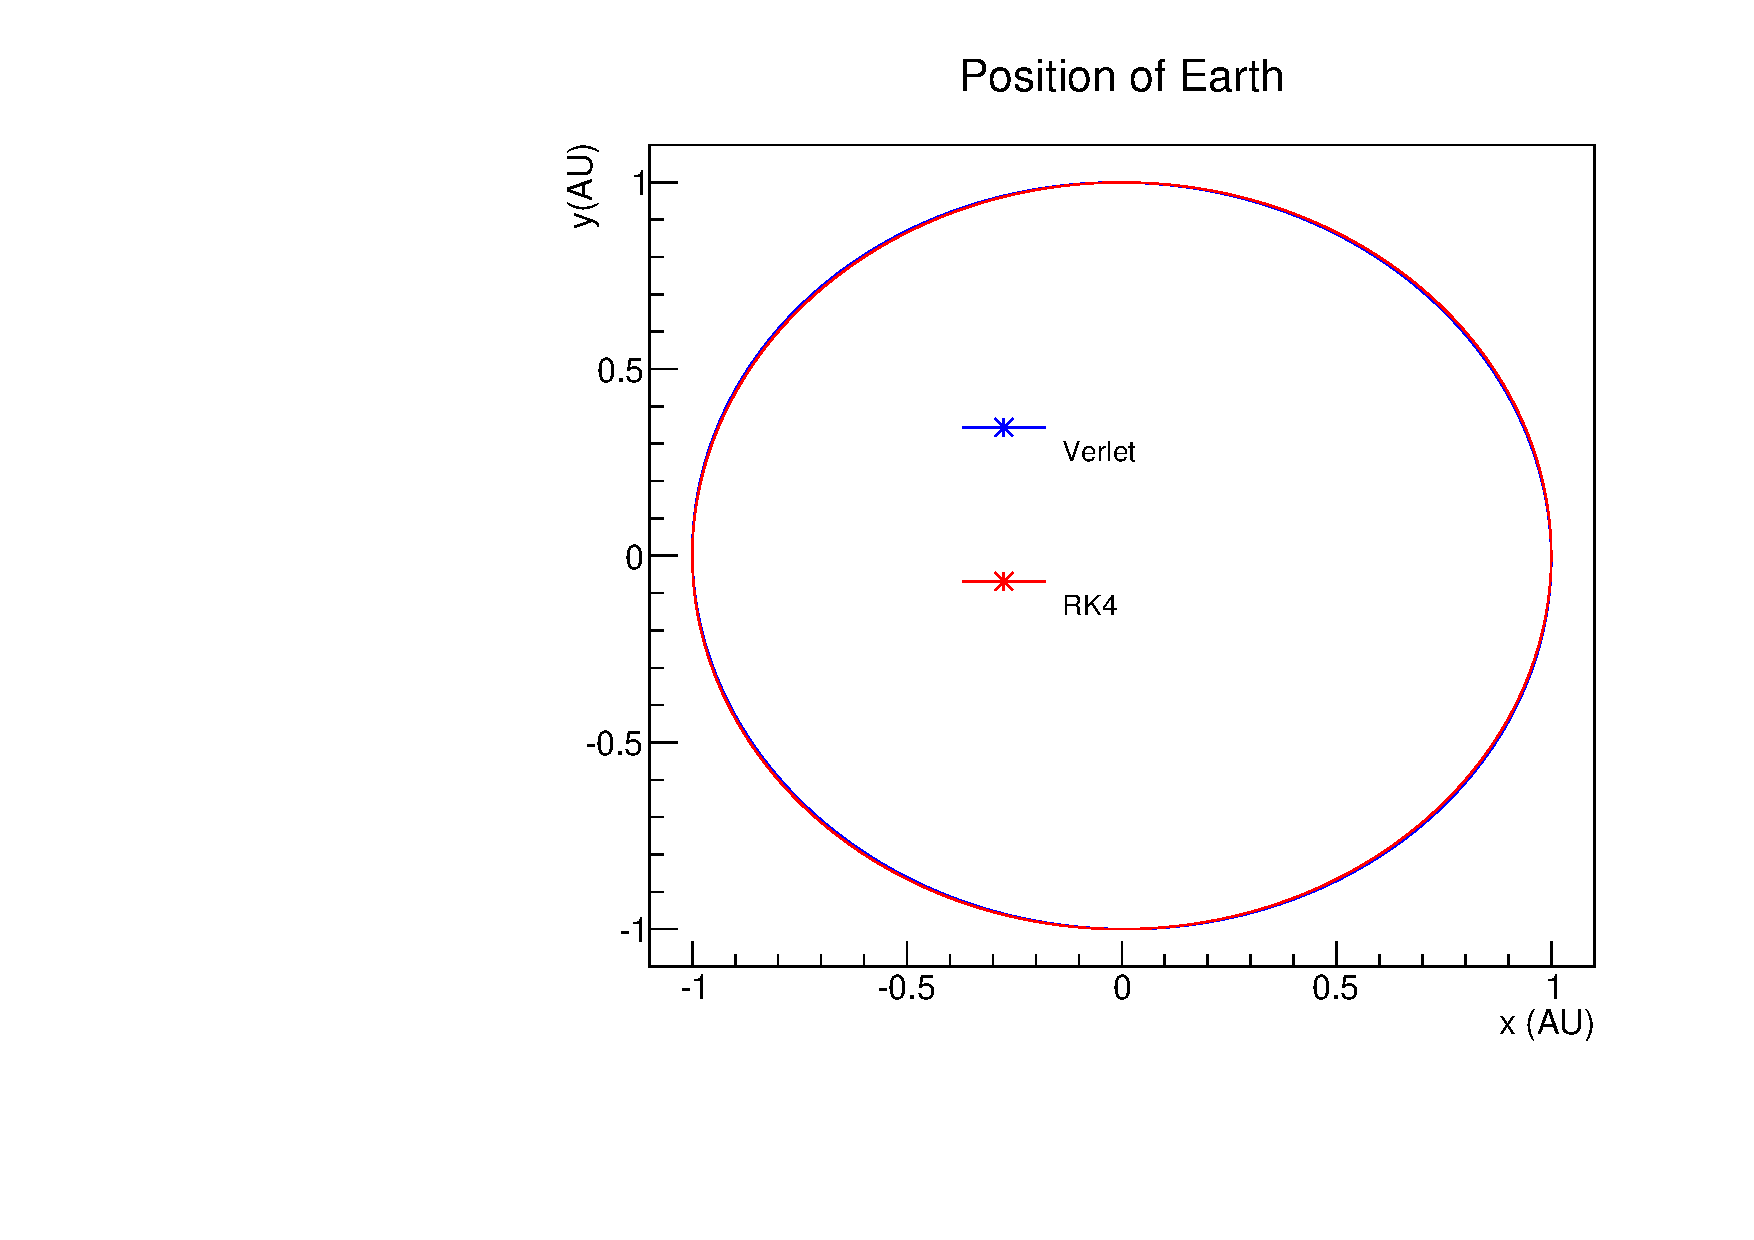
\includegraphics[width=0.47\textwidth]{plots/earth_pos_very_long.png}
\end{subfigure}
\begin{subfigure}
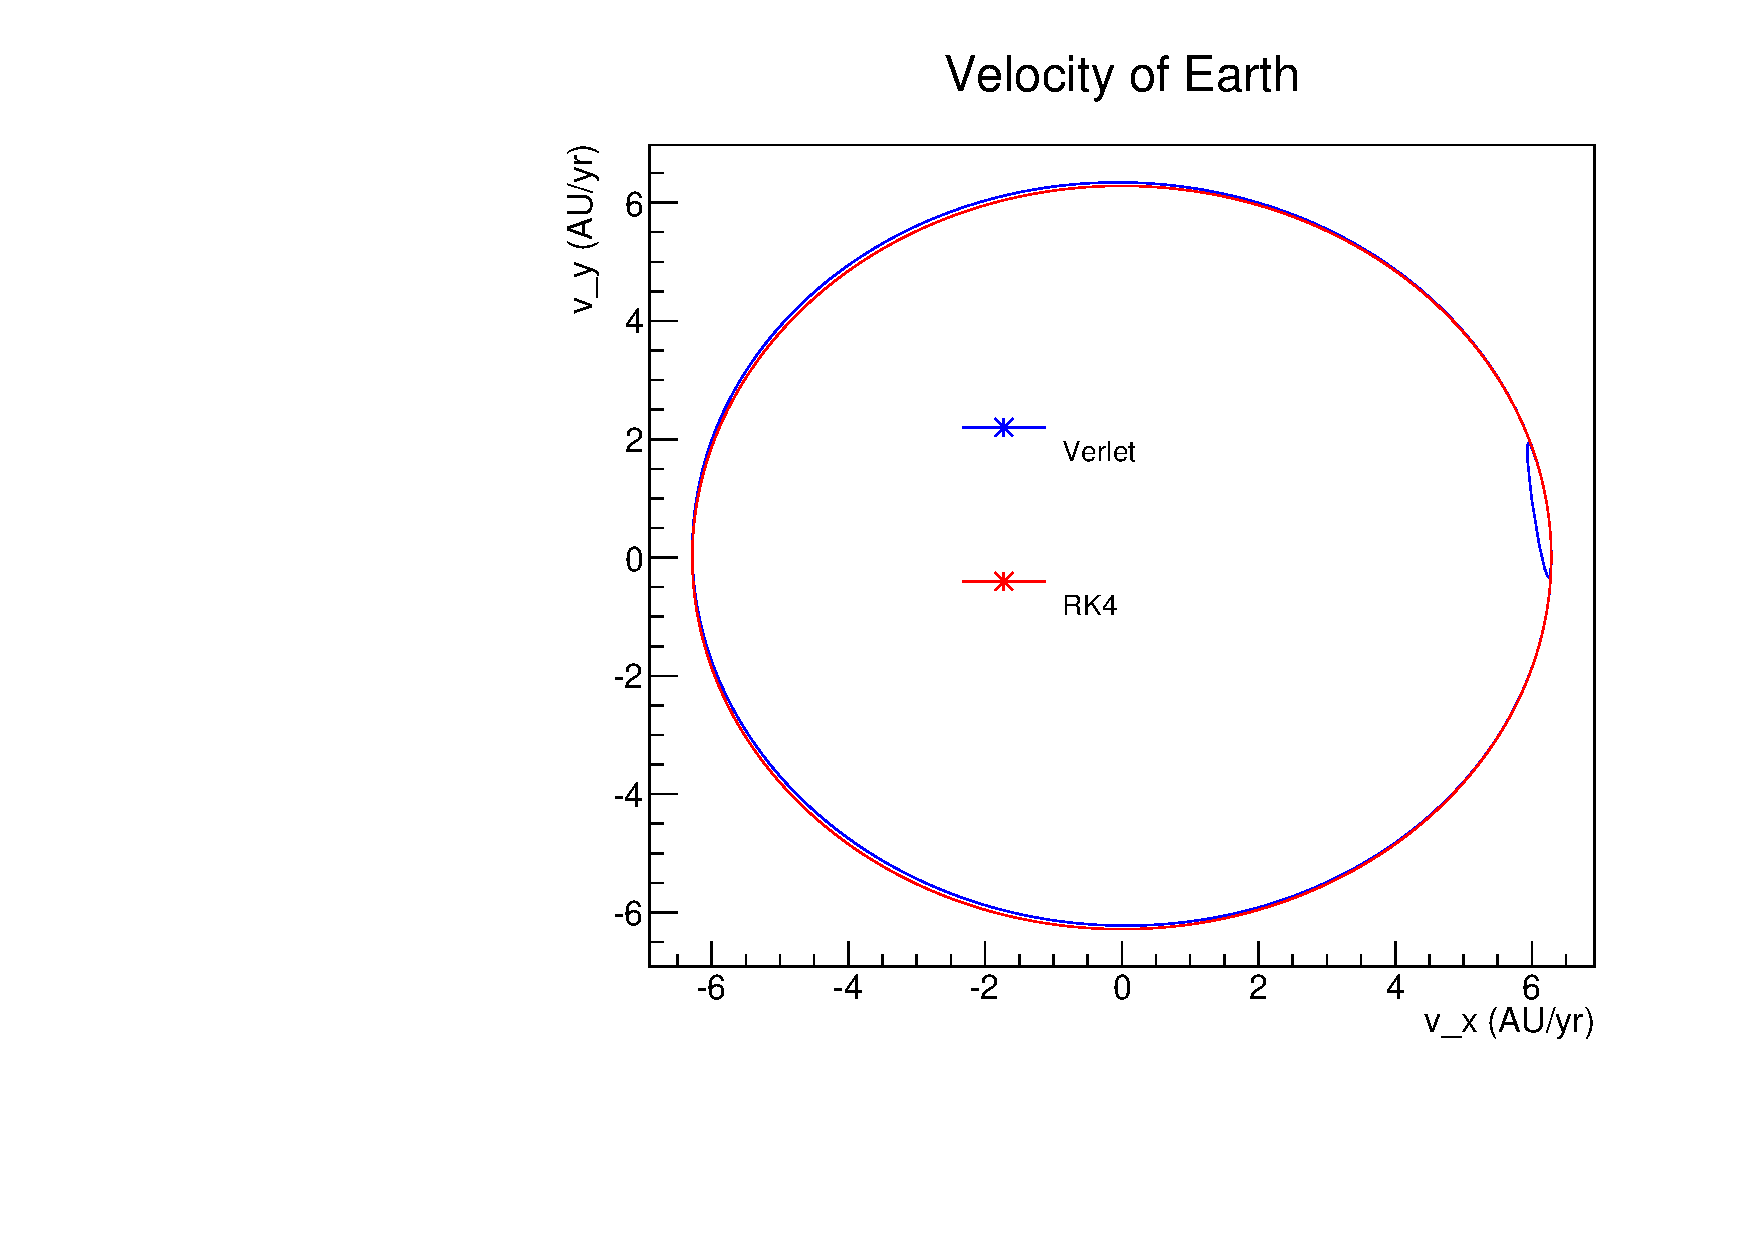
\includegraphics[width=0.47\textwidth]{plots/earth_vel_very_long.png}
\end{subfigure}
\caption{The position and velocity over 3000 years with 1,000,000 steps.  A slight instability is observed in the Verlet velocity solutions.}
\label{fig:2}
\end{center}
\end{figure}

\begin{figure}[h]
\begin{center}
\begin{subfigure}
\includegraphics[width=0.47\textwidth]{plots/earth_pos_long.png}
\end{subfigure}
\begin{subfigure}
\includegraphics[width=0.47\textwidth]{plots/earth_vel_long.png}
\end{subfigure}
\caption{The position and velocity over 300 years with 10000 steps.  We see that the instability with fewer steps per year is much more pronounced than in Fig.~\ref{fig:2}.}
\label{fig:3}
\end{center}
\end{figure}

\par Another test performed was designed to check the stability of both arguments for various step sizes or number of steps. For this test, we looked at the performance of both the Verlet and RK4 algorithms over the course of one year for various step sizes between 2 and 50 (noting from Fig.~\ref{fig:1} that both the Verlet and RK4 algorithms are stable over one year for step size 100.  In Fig.~\ref{fig:4}, we see that, for small step size, the position Verlet algorithm is very unstable.  The orbits are not actually even closed over the course of one year.  However, at 5 steps, the orbit closes (although is not particularly nice), and the orbit finally stabilizes around 10 steps.  The velocity Verlet algorithm forms a closed curve even at 2 steps, but does not become fully stable until between 20 and 50 steps.  This indicates that the velocity Verlet algorithm may require more steps in order to be accurate than the position algorithm (which further validates our hypothesis that more steps may be required for longer times).  

\begin{figure}[h]
\begin{center}
\begin{subfigure}
\includegraphics[width=0.47\textwidth]{plots/pos_nstep_check_verlet.png}
\end{subfigure}
\begin{subfigure}
\includegraphics[width=0.47\textwidth]{plots/pos_nstep_check_rk4.png}
\end{subfigure} \\
\begin{subfigure}
\includegraphics[width=0.47\textwidth]{plots/vel_nstep_check_verlet.png}
\end{subfigure}
\begin{subfigure}
\includegraphics[width=0.47\textwidth]{plots/vel_nstep_check_rk4.png}
\end{subfigure} 
\caption{Checking the stability of the RK4 and Verlet algorithms with varying step sizes over the course of one year.}
\label{fig:4}
\end{center}
\end{figure}

\par The RK4 algorithm has a slightly different step number dependence.  The position RK4 algorithm is not as wildly non-elliptical as the Verlet algorithm even at very small numbers of steps, but doesn't fully stabilize until about 10 steps.  A very similar behavior is observed for the velocity RK4 algorithm.  This similarity (compared with the distinctions between the Verlet algorithm velocity and position results) is likely due to the fact that the velocity and position RK4 algorithms are identical (excepting the function being used to evaluate), whereas the velocity and position Verlet algorithms are slightly different and cannot be evaluated simultaneously.
\par A final test which was performed was designed to check that each algorithm conserved potential, kinetic, and total energy and angular momentum.  Because we assume a circular orbit, we should have a constant radius, which implies that the potential and kinetic energies should be individually conserved (the potential depends only on the radius of the planet from the sun and thus, because total energy must always be conserved, kinetic energy must, in this case, be independently conserved).  Angular momentum should also be conserved because there is no linear motion in the system, and total momentum is always conserved.  
\par We checked these expected conserved quantities again over the course of one year for 100 steps.  We found that generally the RK4 algorithm had better results.  In particular, as shown in Table~\ref{tab:conserve}, the RK4 algorithm is off only by a fraction of a percent whereas the Verlet algorithm is off by about 10\% in every quantity. The variation in these quantities is shown in Fig.~\ref{fig:5}  However, as the time and number of steps increased (particularly as the number of steps increased), it was found that the Verlet algorithm became more accurate.  For example, at 300 years and 100000 steps, the largest percent difference of the conserved quantities was under 5\%.

\begin{figure}[h]
\begin{center}
\begin{subfigure}
\includegraphics[width=0.47\textwidth]{benchmarks/kinetic.png}
\end{subfigure}
\begin{subfigure}
\includegraphics[width=0.47\textwidth]{benchmarks/potential.png}
\end{subfigure} \\
\begin{subfigure}
\includegraphics[width=0.47\textwidth]{benchmarks/total_energy.png}
\end{subfigure}
\begin{subfigure}
\includegraphics[width=0.47\textwidth]{benchmarks/angular_mom.png}
\end{subfigure} 
\caption{Checking that various expected conserved quantities are actually conserved over the course of one year with 100 steps for the RK4 and Verlet algorithms.}
\label{fig:5}
\end{center}
\end{figure}

\begin{table}[h]
\centering
\begin{tabular}{c|c|c|c|c}
& Kinetic Energy & Potential Energy & Total Energy & Angular Momentum \\ \hline
Verlet & 15.068\% & 3.092\% & 7.104\% & 3.100\% \\
RK4 & 8.456$\times10^{-6}$ & 4.228$\times10^{-6}$ & 2.514$\times10^{-13} & 8.456$\times10^{-6}$ 
\end{tabular}
\caption{The percent difference between the maximum and minimum of the expected conserved quantities for the Verlet and RK4 algorithms in the case of the idealized earth-sun model.}
\label{tab:conserve}
\end{table}

\par We next tried to use our algorithms to calculate a convenient quantity -- the escape velocity -- of a planet at a distance of 1 AU from the sun (eg. earth).  To do this, we started with our ideal earth-sun system with a circular orbit.  We then increased our velocity by a small amount until the planet was not at the same distance from the sun after a year of revolution (see \texttt{partd()} and \texttt{partd\_precise()} in \texttt{project3.C}).  We found that the escape velocity was 100.531 AU/yr, and that it was independent of the mass of the planet.  This is because the escape velocity occurs where the potential energy is equal to the kinetic energy.  That is, 

$$
\frac{GM_{\odot}m_{p}}{r}=\frac{1}{2}m_{p}v_{e}^{2}
$$

\noindent or

\begin{equation}
\label{eq:escape}
v_{e} = \sqrt{\frac{2GM_{\odot}}{r}}.
\end{equation}

\noindent From Eq.~\ref{eq:escape}, it is clear that the escape velocity should not be dependent on the mass of the planet (or other object) in orbit around the sun, but just on the mass of the sun and the distance from the sun.  In this case, then, we have

$$
v_{e} = \sqrt{\frac{8\pi^{2}}{1}} = 8.89 \frac{AU}{yr}
$$

\noindent Clearly, then, our calculation of the final escape velocity was incorrectly done within the code.  This is something which it would be nice to investigate further.
\par Once we were satisfied that the basic algorithms were working, we decided to add a second planet -- Jupiter -- to the system.  Assuming the orbits of the earth and Jupiter to be coplanar (in the $x$-$y$ direction), we determined the orbits and velocities of Earth and Jupiter assuming the sun to be at the origin in \texttt{parteandf()} of \texttt{project3.C}.  The results for 500 steps over 10 years are shown in Fig.~\ref{fig:6}.  We can see that all of the results are quite reasonable -- elliptical/circular orbits around a stationary sun at the origin.  With a longer time as well we see that the algorithms are fairly stable.  The plots in  Fig.~\ref{fig:7} are made with 100000 steps over 100 years.  We see that the velocity Verlet algorithm is quite stable in spite of some oscillatory motion from the position algorithm.  The same holds true for the RK4 algorithm.

\begin{figure}[h]
\begin{center}
\begin{subfigure}
\includegraphics[width=0.47\textwidth]{plots/jupiter_only_verlet_pos.png}
\end{subfigure}
\begin{subfigure}
\includegraphics[width=0.47\textwidth]{plots/jupiter_only_verlet_vel.png}
\end{subfigure} \\
\begin{subfigure}
\includegraphics[width=0.47\textwidth]{plots/jupiter_only_rk4_pos.png}
\end{subfigure}
\begin{subfigure}
\includegraphics[width=0.47\textwidth]{plots/jupiter_only_rk4_vel.png}
\end{subfigure} 
\caption{Adding Jupiter to the Earth-sun system and computing the positions and velocities using the RK4 and Verlet algorithms for 500 steps over 10 years.}
\label{fig:6}
\end{center}
\end{figure}

\begin{figure}[h]
\begin{center}
\begin{subfigure}
\includegraphics[width=0.47\textwidth]{plots/jupiter_only_long_verlet_pos.png}
\end{subfigure}
\begin{subfigure}
\includegraphics[width=0.47\textwidth]{plots/jupiter_only_long_verlet_vel.png}
\end{subfigure} \\
\begin{subfigure}
\includegraphics[width=0.47\textwidth]{plots/jupiter_only_long_rk4_pos.png}
\end{subfigure}
\begin{subfigure}
\includegraphics[width=0.47\textwidth]{plots/jupiter_only_long_rk4_vel.png}
\end{subfigure} 
\caption{Adding Jupiter to the Earth-sun system and computing the positions and velocities using the RK4 and Verlet algorithms for 100000 steps over 100 years to check the stability over time.}
\label{fig:7}
\end{center}
\end{figure}

\par We next investigated the stability of the algorithms for various step sizes.  We looked specifically at 50 years with numbers of steps between 500 and 1000.  We found that, for 500 steps, the position and velocity of Earth using RK4 was highly unstable while those for Verlet were more stable (see Fig.~\ref{fig:8}).  By 1000 steps, however, the orbits seem quite stable for both methods (although there did seem to be some instability still in the velocity Verlet algorithm).  Instability in the RK4 algorithm persisted until around 700 steps.

\begin{figure}[h]
\begin{center}
\begin{subfigure}
\includegraphics[width=0.47\textwidth]{plots/jupiter_only_long_500steps_verlet_pos.png}
\end{subfigure}
\begin{subfigure}
\includegraphics[width=0.47\textwidth]{plots/jupiter_only_long_500steps_verlet_vel.png}
\end{subfigure} \\
\begin{subfigure}
\includegraphics[width=0.47\textwidth]{plots/jupiter_only_long_500steps_rk4_pos.png}
\end{subfigure}
\begin{subfigure}
\includegraphics[width=0.47\textwidth]{plots/jupiter_only_long_500steps_rk4_vel.png}
\end{subfigure} 
\caption{Adding Jupiter to the Earth-sun system and computing the positions and velocities using the RK4 and Verlet algorithms for 500 steps over 50 years to check the stability over time.}
\label{fig:8}
\end{center}
\end{figure}

\par We next looked at what happened when we made Jupiter heavier.  We started by making Jupiter 10 times its actual mass.  Starting with 750 steps (Fig.~\ref{fig:9}), we slowly increased the number of steps until we had achieved a stable orbit.   With this approach, we found that we tried as many as 10000 steps between 0 and 50 years, and never achieved a stable orbit.  It was impractical to attempt more steps due to computing time, and so we assume that no such stable orbit exists.  We can make a similar statement about the orbit for the planets if Jupiter is 1000 times its actual mass, shown in Fig.~\ref{fig:10}, which we checked with 2000 steps over 50 years.

\begin{figure}[h]
\begin{center}
\begin{subfigure}
\includegraphics[width=0.47\textwidth]{plots/jupiter10_only_long_750steps_verlet_pos.png}
\end{subfigure}
\begin{subfigure}
\includegraphics[width=0.47\textwidth]{plots/jupiter10_only_long_750steps_verlet_vel.png}
\end{subfigure} \\
\begin{subfigure}
\includegraphics[width=0.47\textwidth]{plots/jupiter10_only_long_750steps_rk4_pos.png}
\end{subfigure}
\begin{subfigure}
\includegraphics[width=0.47\textwidth]{plots/jupiter10_only_long_750steps_rk4_vel.png}
\end{subfigure} 
\caption{Investigating the effect of making Jupiter 10 times more massive than it actually is on the orbit of earth around the sun in the three-body system.}
\label{fig:9}
\end{center}
\end{figure}

\begin{figure}[h]
\begin{center}
\begin{subfigure}
\includegraphics[width=0.47\textwidth]{plots/jupiter1000_only_long_2000steps_verlet_pos.png}
\end{subfigure}
\begin{subfigure}
\includegraphics[width=0.47\textwidth]{plots/jupiter1000_only_long_2000steps_verlet_vel.png}
\end{subfigure} \\
\begin{subfigure}
\includegraphics[width=0.47\textwidth]{plots/jupiter1000_only_long_2000steps_rk4_pos.png}
\end{subfigure}
\begin{subfigure}
\includegraphics[width=0.47\textwidth]{plots/jupiter1000_only_long_2000steps_rk4_vel.png}
\end{subfigure} 
\caption{Investigating the effect of making Jupiter 1000 times more massive than it actually is on the orbit of earth around the sun in the three-body system.}
\label{fig:10}
\end{center}
\end{figure}

\par We next investigated the movement of the planets about the center of mass of the system.  To do this, we computed the center of mass and set this as the origin.  We wanted the center of mass to be a stationary point, so we needed to adjust the velocity of the sun.  We know that the velocity $v_{com}$ of the center of mass is given by 

$$
v_{com} = \frac{\sum_{p} m_{p}v_{p}}{\sum_{p} m_{p}}
$$

\noindent This indicates that the velocity of the sun should be

\begin{equation}
\label{eq:suncom}
v_{sun} = -\frac{\sum_{p\neq sun}m_{p}v_{p}}{m_{sun}}.
\end{equation}

\noindent So we set the velocity of the sun to be as in Eq.~\ref{eq:suncom} and looked at the movement of the planets for 1000 steps over 10 years as shown in Fig.~\ref{fig:11}.  We see that in fact the sun moves very little -- an almost negligible amount -- with these restrictions.

\begin{figure}[h]
\begin{center}
\begin{subfigure}
\includegraphics[width=0.47\textwidth]{plots/jupiter_only_com_verlet_pos.png}
\end{subfigure}
\begin{subfigure}
\includegraphics[width=0.47\textwidth]{plots/jupiter_only_com_verlet_vel.png}
\end{subfigure} \\
\begin{subfigure}
\includegraphics[width=0.47\textwidth]{plots/jupiter_only_com_rk4_pos.png}
\end{subfigure}
\begin{subfigure}
\includegraphics[width=0.47\textwidth]{plots/jupiter_only_com_rk4_vel.png}
\end{subfigure} 
\caption{The three-body problem solved over 10 years with 1000 steps with the origin at the center of mass of the system and the initial velocity of the sun set as in Eq.~\ref{eq:suncom}.}
\label{fig:11}
\end{center}
\end{figure}

\par Finally, we looked at solving the full solar system problem.  Here we investigated the motion over 100 years with 10000 steps, first with the sun as the origin, as shown in Fig.~\ref{fig:12}, and then with the center of mass at the origin and the sun's velocity set as in Eq.~\ref{eq:suncom}.  In both cases, the initial velocities for each planet were assumed to be the average velocity of the planet around the sun.  These numbers and the masses and average distances from the sun were taken from [6].
\par We can see that, in Fig.~\ref{fig:12}, the orbits seem stable and elliptical, as expected.  The only small instability comes from the RK4 algorithm, where we see that the velocity of mercury has some fluctuations as time progresses (as evidenced by the thicker velocity ring).  This is somewhat surprising as some sources [5] suggest that only a step size of 0.5 days should be needed to observe stability, and our step size was $\sim0.2$ days.  However, it is not clear which integrating technique this source used and, as our Verlet algorithm does indicate stability, it is fairly safe to say that this instability observed may be a step size problem or a small bug in the code.  
\par In Fig.~\ref{fig:13}, we solve the same problem taking the origin to be the center of mass of the system and solving for the initial velocity of the sun as in Eq.~\ref{eq:suncom}.  We see here that, as in Fig.~\ref{fig:12}, the solutions seem to be quite stable over time excepting again the velocity of Mercury which shows the same possible instabilities as were seen in the solution with a stationary sun at the origin.

\begin{figure}[h]
\begin{center}
\begin{subfigure}
\includegraphics[width=0.47\textwidth]{plots/milky_way_full_100yrs_verlet_pos.png}
\end{subfigure}
\begin{subfigure}
\includegraphics[width=0.47\textwidth]{plots/milky_way_full_100yrs_verlet_vel.png}
\end{subfigure} \\
\begin{subfigure}
\includegraphics[width=0.47\textwidth]{plots/milky_way_full_100yrs_rk4_pos.png}
\end{subfigure}
\begin{subfigure}
\includegraphics[width=0.47\textwidth]{plots/milky_way_full_100yrs_rk4_vel.png}
\end{subfigure} 
\caption{The solution to the solar system over 100 years with 10000 steps with the sun at the origin.}
\label{fig:12}
\end{center}
\end{figure}

\begin{figure}[h]
\begin{center}
\begin{subfigure}
\includegraphics[width=0.47\textwidth]{plots/milky_way_full_com_verlet_pos.png}
\end{subfigure}
\begin{subfigure}
\includegraphics[width=0.47\textwidth]{plots/milky_way_full_com_verlet_vel.png}
\end{subfigure} \\
\begin{subfigure}
\includegraphics[width=0.47\textwidth]{plots/milky_way_full_com_rk4_pos.png}
\end{subfigure}
\begin{subfigure}
\includegraphics[width=0.47\textwidth]{plots/milky_way_full_com_rk4_vel.png}
\end{subfigure} 
\caption{The solution to the solar system over 100 years with 10000 steps with the center of mass as the origin.}
\label{fig:13}
\end{center}
\end{figure}
\section{Conclusions}
\label{sec:conclusions}

Overall, this project was fairly successful.  We were able to create a fully object-oriented C++ code which could work with planets and solar systems and calculate the positions and velocities of those planets in orbit around the sun.  We were able to find relative stability in the orbits of the planets, as expected, in both the cases of the sun stationary at the center of the system and with the center of mass of the system as the origin and the sun moving in such a way (Eq.~\ref{eq:suncom}) as to keep the center of mass stationary.  However, there are several further tests which may be performed on the algorithms and which may shed more light on the apparent fluctuations in Mercury's velocity as it orbits around the sun as part of the full solar system.
\par The first and probably most enlightening study we might perform is a further investigation into the dependence of the stability of the Verlet and RK4 algorithms on step size and length of time.  It was observed throughout the course of the project that both algorithms, but particularly the RK4 algorithm, required a very small step size in order to accurately compute the positions and velocities of the planets.  It would be interesting to do a study on what the minimum number of steps would be for integration for larger systems specifically.  
\par Along these lines, it would also be useful to work on optimizing the code.  One of the main limitations in what was studied in this project was computation time.  In particular, the RK4 algorithm took significantly longer to run than the Verlet algorithm.  This makes sense because, for each step, the RK4 algorithm calculates four floating point quantites which must be further combined into the solution.  This gave us only 2 flops per quantity (ie. 8 flops to calculate the $k$'s) for the positions.  However, this number was quite a bit larger for the velocities because each planet required 6 flops per $k$ based on the function used in the integration.  With 11 planets, we had 66 flops per $k$.  This means that. due to computational time, we were unable to do any more than what was discussed in Section~\ref{sec:results}.The Verlet algorithm is not as flop-heavy, but still requires $\sim9$ flops per planet for the position calculations and about 11 for the velocity calculations.  This requires a very high computation time as well.
\par We would also like to spend more time working on the calculation of the escape velocity.  As discussed in Section~\ref{sec:results}, our calculation of this quantity was inconsistent with expected values.  It would be very useful to have more time to devote to this problem, as it provides a very convenient check that the algorithms are working properly.

\section{Bibliography}
\label{sec:bib}

\begin{enumerate}

\item Brun, Rene, and Fons Rademakers. "ROOT - An Object Oriented Data Analysis Framework." \textit{Nuclear Instruments and Methods in Physics Research A} 389 (1997): 81-86. Web.
\item Drueke, Elizabeth A. \textit{Programming a Linear Algebra Solution to the Poisson Equation.} Rep. N.p.: n.p., n.d. Print.
\item Drueke, Elizabeth A. \textit{Programming a Linear Algebra Solution to the Problem of Two Electrons Trapped in a Spherical Harmonic Oscillator Well.} Rep. N.p.: n.p., n.d. Print.
\item Hjorth-Jensen, Morten. \textit{Computational Physics}. N.p.: Department of Physics, U of Oslo, n.d. Print.
\item Laskar, Jacques. "Stability of the Solar System." \textit{Scholarpedia.} Scholarpedia, 31 Oct. 2014. Web. 12 Apr. 2016. $<$http://www.scholarpedia.org/article/Stability\_of\_the\_solar\_system$>$.
\item "Planetary Fact Sheet - Metric." \textit{Planetary Fact Sheet.} NASA, n.d. Web. 12 Apr. 2016. $<$http://nssdc.gsfc.nasa.gov/planetary/factsheet/$>$.

\end{enumerate}

\end{document}